\documentclass[10pt,a4paper]{article}

% ---- arXiv-style preamble ----
\usepackage[margin=0.95in]{geometry}
\usepackage[utf8]{inputenc}
\usepackage[T1]{fontenc}
\usepackage{lmodern}
\usepackage{microtype}
\usepackage{amsmath,amssymb,amsthm}
\usepackage{booktabs}
\usepackage{multirow}
\usepackage{array}
\usepackage{graphicx}
\usepackage{xcolor}
\usepackage{subcaption}
\usepackage{url}
\usepackage[numbers,sort&compress]{natbib}
\usepackage[colorlinks=true,linkcolor=black,citecolor=blue,urlcolor=blue]{hyperref}
\usepackage{authblk}
\usepackage{enumitem}
\usepackage{caption}
\usepackage{titlesec}

% Tighter spacing typical of arXiv preprints
\titlespacing*{\section}{0pt}{1.3ex plus .2ex minus .2ex}{0.9ex plus .1ex}
\titlespacing*{\subsection}{0pt}{1.1ex plus .2ex minus .2ex}{0.6ex plus .1ex}
\titlespacing*{\paragraph}{0pt}{0.7ex plus .1ex minus .1ex}{0.6em}
\setlength{\parskip}{0.25ex}
\captionsetup{font=small,labelfont=bf}

\renewcommand{\abstractname}{\normalsize\textsc{Abstract}}
\renewcommand{\baselinestretch}{1.03}

% ---- Title ----
\title{\textbf{\large AeroGraph: Hybrid Graph--Vector Retrieval with\\ Dual-Judge Evaluation over Aviation Safety Narratives}}

\author{Aryan Dhawan}
\affil{\small University of Waterloo \quad \texttt{aryansdhawan@gmail.com}}

\date{\small\today}

\begin{document}
\maketitle

% ---------------------------------------------------------------
% Abstract
% ---------------------------------------------------------------
\begin{abstract}
\small
Multi-hop causal reasoning over aviation safety incident reports is a task at
which flat dense retrieval consistently underperforms. Relevant evidence is
distributed across many short narratives that share only a chain of entities.
We present \textsc{AeroGraph}, a hybrid retrieval system that constructs a
domain-specific knowledge graph from 2{,}000 real NASA Aviation Safety Reporting
System (ASRS) reports via LLM-based entity and relation extraction guided by a
ten-type aviation ontology, and fuses four retrieval signals (dense vector,
sparse BM25, Personalized PageRank, and Leiden-community summaries) through
Reciprocal Rank Fusion. Raw extraction yields $29{,}244$ entities and $43{,}505$
relations; taxonomy-based canonicalization (HFACS, ICAO aircraft and airport
codes, flight phases) and synonym expansion reduce this to $23{,}948$ entities
and $48{,}479$ relations across $186$ weakly connected components. We evaluate
six retrieval systems on a $50$-query benchmark under two independent judges:
a local \texttt{qwen2.5:7b} and Claude Sonnet. The four-signal fusion attains
the highest precision@10 ($0.210$, $+84\%$ over a vector-only baseline at
$0.114$) and the highest faithfulness under both judges, winning $62$ to $72\%$
of blind pairwise answer-quality comparisons against single-signal baselines.
Personalized PageRank alone matches the full hybrid on retrieval precision
within $5\%$ (P@10 $=0.200$) but loses decisively on pairwise preference. This
gap indicates that signal \emph{diversity}, rather than the top-rank precision
of any single signal, is the dominant driver of answer quality. Claude scores
$0.2$ to $0.4$ lower than Ollama on absolute faithfulness, a systematic gap;
system rankings are preserved across judges. Code, taxonomy data, and per-query
judge scores are released at
\url{https://github.com/Aryan95614/AeroGraph}.
\end{abstract}

\vspace{0.3ex}

% ---------------------------------------------------------------
% 1. Introduction
% ---------------------------------------------------------------
\section{Introduction}
\label{sec:intro}

The U.S. Federal Aviation Administration holds more than $15{,}000$ public
near-miss reports annually, a figure that has roughly doubled over the past
decade. Each report is a short, unstructured narrative written by a pilot, air
traffic controller, or maintenance technician describing an incident and its
contributing factors. Individually, reports are low value: they describe events
that almost happened. Collectively, they encode the operational precursors of
serious accidents. The January 2025 mid-air collision near Reagan National
Airport, which killed 67 people, involved contributing factors (high-density
traffic, altitude-clearance ambiguity, visual-approach workload) that appear
repeatedly in ASRS narratives filed over the preceding decade.

Surfacing those patterns at scale requires retrieval that is both
recall-sensitive (finding the handful of relevant reports among tens of
thousands) and capable of multi-hop reasoning (combining evidence from reports
that share no vocabulary but do share a chain of entities). Flat dense
retrieval, the standard baseline, fails on both counts. It surfaces
surface-form similar passages while missing semantically related reports that
describe the same causal chain with different terminology, and it provides no
mechanism for following an entity through a graph of co-occurrences.

This paper presents \textsc{AeroGraph}, an end-to-end hybrid retrieval system
that addresses these failure modes by combining four complementary retrieval
signals over a structured knowledge graph. Our contributions are:

\begin{itemize}[leftmargin=1.2em,itemsep=1pt,topsep=2pt]
\item An open implementation of three recent hybrid-retrieval paradigms
(Microsoft GraphRAG \citep{edge2024graphrag}, HippoRAG's Personalized
PageRank retrieval \citep{gutierrez2024hipporag}, and Agarwal-style
taxonomy-normalized entity resolution \citep{agarwal2022aviation}), unified
into a single 4-way RRF fusion.
\item A $2{,}000$-report benchmark with $50$ annotated queries (single-hop,
multi-hop, comparative) evaluated across six retrieval systems with
$95\%$ confidence intervals and Wilcoxon signed-rank tests. The benchmark,
all per-query outputs, and all judge scores are released.
\item A dual-judge evaluation protocol (local Ollama \texttt{qwen2.5:7b} plus
Claude Sonnet) that exposes a systematic $0.2$ to $0.4$ faithfulness gap
between judges on identical outputs. Rankings are largely preserved;
absolute numbers are judge-sensitive.
\item An empirical finding underexplored in the RAG literature: Personalized
PageRank alone nearly matches the full 4-way fusion on retrieval precision
(P@10 $0.200$ vs $0.210$) but loses decisively on blind pairwise preference.
Signal \emph{diversity}, not any single signal's top rank, is the dominant
driver of final answer quality.
\end{itemize}

% ---------------------------------------------------------------
% 2. Related Work
% ---------------------------------------------------------------
\section{Related Work}
\label{sec:related}

\paragraph{Retrieval-augmented generation.}
\citet{lewis2020rag} established the retrieve-then-read pattern that underlies
most open-domain QA systems. Subsequent work extends the basic architecture.
Fusion-in-Decoder \citep{izacard2021fid} encodes passages independently before
decoder fusion. RETRO \citep{borgeaud2022retro} scales retrieval to
trillion-token datastores. HyDE \citep{gao2023hyde} retrieves against a
hypothetical answer to bridge query-document vocabulary gaps. Self-RAG
\citep{asai2024selfrag} trains a model to decide when and what to retrieve.
A persistent limitation is that flat retrieval over independent chunks
struggles with multi-hop reasoning \citep{trivedi2023ircot}, since the
evidence needed for such queries is distributed across documents that do not
individually match the query.

\paragraph{Graph-based retrieval and GraphRAG.}
Knowledge-graph augmentation of language models predates modern RAG.
\citet{sun2018graftnet} and \citet{yasunaga2021qagnn} integrate structured
knowledge-base traversal with language-model reasoning for commonsense QA.
The term \emph{GraphRAG} was established by \citet{edge2024graphrag}, whose
two-stage pipeline (LLM-based entity and relation extraction followed by
Leiden-algorithm community detection \citep{traag2019leiden} and hierarchical
summarization) yields substantial gains on global sense-making queries over
corpora of news and podcast transcripts. \citet{gutierrez2024hipporag} propose
HippoRAG, a neurobiologically inspired alternative that replaces community
summaries with Personalized PageRank over an entity knowledge graph and
attains strong multi-hop QA performance. Our hybrid retriever follows HippoRAG
in using PPR as a core signal, follows GraphRAG in using community summaries
for global queries, and adds dense vector and sparse BM25 as complementary
signals within a single Reciprocal Rank Fusion \citep{cormack2009rrf} pipeline.

\paragraph{NLP for aviation safety.}
ASRS has been studied primarily through text classification and topic modeling
\citep{kuhn2018asrs,rose2015asrs}. Formal taxonomies such as HFACS
\citep{shappell2001hfacs} and ICAO occurrence categories \citep{icao2016doc9859}
provide the canonical vocabulary for human and technical contributing factors.
\citet{agarwal2022aviation} show that taxonomy-normalized extraction
substantially improves downstream analytics. We adopt this insight directly,
treating HFACS Level-2 categories and ICAO aircraft and airport codes as
canonical lookup targets during entity resolution.

\paragraph{LLM-based information extraction.}
LLMs attain competitive zero-shot NER performance \citep{wei2023llmie} but
suffer on fine-grained entity distinctions and introduce fragmentation: the
same real-world concept is extracted as multiple distinct nodes under slight
surface-form variation. \citet{wadhwa2023relations} document the same
tradeoff for relation extraction. We mitigate fragmentation with
ontology-constrained prompting, number-aware fuzzy deduplication, and a
three-tier taxonomy resolution pass (exact match, then \texttt{rapidfuzz}
edit-distance, then sentence-transformer embedding similarity) following
\citet{agarwal2022aviation}.

\paragraph{RAG evaluation.}
RAGAS \citep{es2024ragas} decomposes RAG evaluation into faithfulness, answer
relevance, context precision, and context recall. LLM-as-judge is now
standard \citep{zheng2024judgingllm}, with documented position, verbosity, and
self-enhancement biases that affect absolute but rarely relative scores. We
adopt RAGAS-style metrics and mitigate self-enhancement bias by evaluating
under two independent judges: one local open-weight model and one frontier
API model.

% ---------------------------------------------------------------
% 3. Dataset and Ontology
% ---------------------------------------------------------------
\section{Dataset and Ontology}
\label{sec:data}

We work with $2{,}000$ ASRS reports sampled from the public
\texttt{elihoole/asrs-aviation-reports} HuggingFace dataset ($38{,}655$ total
records). Each report combines two narrative fields (Reporter~1, Reporter~2)
with structured metadata: ACN (accession number), aircraft make and model,
phase of flight, and anomaly classification. Aircraft strings are normalized
to canonical ICAO designators at ingestion so that \emph{Boeing 737-800},
\emph{B737-800}, and \emph{737} all map to \textsc{B737}. Float-formatted ACNs
are normalized to integers. Reports with fewer than fifty narrative words are
filtered.

\paragraph{Ontology.}
The aviation safety ontology has $10$ node types (\textsc{Aircraft},
\textsc{Event}, \textsc{Phase}, \textsc{Factor}, \textsc{Component},
\textsc{Outcome}, \textsc{Recommendation}, \textsc{ATC\_Facility},
\textsc{Weather}, \textsc{TimePeriod}) and $8$ edge types (\textsc{CAUSED\_BY},
\textsc{CONTRIBUTED\_TO}, \textsc{OCCURRED\_DURING}, \textsc{INVOLVED},
\textsc{RESOLVED\_BY}, \textsc{PRECEDED\_BY}, \textsc{CO\_OCCURRED\_WITH},
\textsc{TEMPORAL\_SEQUENCE}). The ontology is intentionally coarser than
ECCAIRS or CAST: richer taxonomies exceed current LLM extraction reliability
without substantial benefit at our corpus size.

\paragraph{Taxonomy coverage.}
The normalization pass uses five canonical lookup tables totaling $1{,}205$
surface-form aliases: HFACS Level-2 ($19$ categories, $152$ aliases), ICAO
aircraft designators ($37$ types, $215$ aliases), airports ($154$ ICAO codes,
$571$ aliases), weather conditions ($20$ categories, $119$ aliases), and
flight phases ($12$ phases, $100$ aliases). All lookup data ships with the
public repository.

% ---------------------------------------------------------------
% 4. System Design
% ---------------------------------------------------------------
\section{System Design}
\label{sec:system}

\subsection{Entity and Relation Extraction}

Reports are processed in batches of $20$ by Claude Sonnet with an
ontology-constrained structured-JSON prompt. The system message specifies the
$10$ node types and $8$ edge types. The user message contains one report's
narrative plus metadata. Retry logic (exponential backoff via
\texttt{tenacity}) handles API rate limits. Extracted results are cached, so
re-runs are idempotent.

Post-extraction normalization has three stages:
\begin{enumerate}[leftmargin=1.2em,itemsep=1pt,topsep=1pt]
\item \textbf{Name canonicalization.} Lowercasing, whitespace collapse,
trailing-punctuation removal, aviation abbreviation expansion.
\item \textbf{Fuzzy deduplication.} Within each entity type, names with
\texttt{SequenceMatcher} similarity above $0.85$ are merged. A number-aware
guard prevents merges that differ only by a numeric identifier:
\emph{engine~1 failure} $\neq$ \emph{engine~2 failure};
\emph{runway~28L} $\neq$ \emph{runway~28R}.
\item \textbf{Taxonomy resolution.} A three-tier cascade (exact match, then
\texttt{rapidfuzz} edit-distance at threshold $85$, then sentence-transformer
cosine similarity at $0.80$) maps extracted entities to canonical HFACS
categories, ICAO codes, and weather and phase identifiers.
\end{enumerate}

\subsection{Knowledge Graph Construction}

Extracted entities and relations merge into a directed graph with
$\textsc{Merge}$ semantics. Nodes key on $(\text{type},
\text{canonical\_name})$; edges on $(\text{source}, \text{target},
\text{type})$. Duplicate edges increment a weight counter and accumulate
report-ID lists. Two interchangeable backends are supported (Neo4j for
production; NetworkX as an in-process fallback) exposing a common query
interface (\texttt{get\_neighbors}, \texttt{get\_causal\_chain},
\texttt{get\_subgraph}, \texttt{get\_temporal\_chain}).

\paragraph{Hub suppression.}
Two-hop BFS expansion skips nodes whose degree exceeds a configurable
threshold (default $200$). Without this guard, high-frequency entities
(common aircraft types, generic events) inflate the neighborhood to include
thousands of weakly related reports.

\paragraph{Graph statistics.}
Raw extraction produces $29{,}244$ entities and $43{,}505$ relations but
$3{,}766$ weakly connected components, of which $3{,}367$ are isolated
nodes. This is a well documented failure mode of LLM extraction. Taxonomy
normalization collapses entities to $23{,}948$ canonical nodes and $48{,}479$
relations, reducing components to $245$. A synonym-edge pass (adding
\textsc{SYNONYM} edges between canonical-to-alias pairs) reduces components
further to $186$. Leiden clustering \citep{traag2019leiden} over the
canonicalized graph yields $311$, $393$, and $296$ communities at three
resolution levels. We precompute LLM summaries for the $100$ largest
communities (mean length $1{,}419$ characters, range $1{,}198$ to $1{,}645$).
These serve as retrieval targets for global queries.

\subsection{Hybrid Retrieval}

Four signals are computed in parallel, then fused.

\paragraph{Dense vector.}
Reports are chunked into $256$-token windows with $128$-token overlap, embedded
with \texttt{sentence-transformers/all-MiniLM-L6-v2} ($384$ dimensions), and
stored in ChromaDB ($4{,}710$ chunks). The top $2k$ chunks are retrieved by
cosine similarity at query time.

\paragraph{Sparse BM25.}
A from-scratch Okapi BM25 implementation ($k_1 = 1.5$, $b = 0.75$) indexes
the same chunk corpus. The inverted index is built at query time from the
ChromaDB corpus with no external library.

\paragraph{Personalized PageRank.}
Query entities are extracted (keyword match against the entity index, with
Claude fallback) and serve as the personalization vector for a PageRank
computation with $\alpha = 0.15$. Nodes are ranked by stationary probability;
reports are scored by summed probability over their constituent entities.

\paragraph{Community summaries.}
For queries classified as global (via a lightweight keyword heuristic), the
$100$ community summaries are scored by BM25 against the query. The top $10$
summaries pass as additional context.

\paragraph{Reciprocal Rank Fusion.}
Signals are fused with RRF \citep{cormack2009rrf}:
\begin{equation}
\text{RRF}(d) = \sum_{s \in \mathcal{S}} \frac{w_s}{k + \text{rank}_s(d)}\,,
\label{eq:rrf}
\end{equation}
where $k = 45$ (tuned from the standard $60$ on a validation split) and
$\mathcal{S} = \{\text{vector}, \text{BM25}, \text{PPR},
\text{community}\}$. Per-signal weights are $w_{\text{vector}} = 1.0$,
$w_{\text{BM25}} = 1.0$, $w_{\text{PPR}} = 1.5$,
$w_{\text{community}} = 1.3$, tuned on a held-out validation subset;
uniform-weight ablations appear in Section~\ref{sec:results}.

\subsection{Answer Generation}

The top-$k$ chunks, PPR-highlighted entities, and applicable community
summaries pass to Claude Sonnet. The system prompt establishes the role of
an aviation safety analyst and instructs the model to cite specific ACN
identifiers, mark unsupported claims as such, and use causal language only
when supported by \textsc{CAUSED\_BY} or \textsc{CONTRIBUTED\_TO} edges.

% ---------------------------------------------------------------
% 5. Experimental Setup
% ---------------------------------------------------------------
\section{Experimental Setup}
\label{sec:setup}

\subsection{Benchmark Queries}

The $50$-query benchmark covers three query types. \emph{Single-hop} factual
queries ($n=20$) test fact retrieval from one report (for example: ``What
weather condition is most commonly associated with go-around decisions?'').
\emph{Multi-hop} causal queries ($n=20$) test reasoning across reports
(``What causal chain links bird strikes to engine failure and subsequent
go-around decisions?''). \emph{Comparative} queries ($n=10$) test
cross-corpus comparison (``Compare contributing factors in B737 vs. A320
engine failure incidents''). Queries were constructed to exercise the ten
entity types and eight edge types of the ontology and are released with the
benchmark artifacts.

\subsection{Retrieval Systems}

Six retrieval configurations are evaluated:
\begin{enumerate}[leftmargin=1.2em,itemsep=1pt,topsep=1pt]
\item \textbf{Vector baseline}: ChromaDB dense-only retrieval.
\item \textbf{BM25}: Sparse-only retrieval over the chunk corpus.
\item \textbf{Graph-Only}: 2-hop BFS neighborhood expansion from query
entities, with report scoring by matched-entity coverage.
\item \textbf{GraphRAG}: Vector plus 2-hop graph fused via RRF, as in
\citet{edge2024graphrag} but without community summaries.
\item \textbf{PPR-Only}: Personalized PageRank on the entity graph,
HippoRAG's core signal \citep{gutierrez2024hipporag}.
\item \textbf{HippoRAG 4-way}: Full $4$-signal RRF fusion
(vector $+$ BM25 $+$ PPR $+$ community summaries).
\end{enumerate}
All systems share the same generation backend (Claude Sonnet with identical
system prompt), isolating retrieval as the experimental variable.

\subsection{Metrics}

\paragraph{Retrieval.} Precision@10, Recall@10, and nDCG@10 against
graph-derived relevance labels. A report $r$ is relevant to query $q$ if
$q$'s extracted entities intersect $r$'s entity set. Hub-node filtering is
applied: entities with degree $> 200$ are excluded from the relevance
computation to prevent trivial matches.

\paragraph{Generation.} Faithfulness and answer relevance are scored by two
independent LLM judges. The \emph{Ollama judge} is a local
\texttt{qwen2.5:7b} model with a strict four-criterion binary rubric
(entity grounding, causal grounding, claim support, no fabrication). The
\emph{Claude judge} is Claude Sonnet with the same rubric on a
$\{0, 0.25, 0.5, 0.75, 1\}$ scale. Causal chain accuracy is scored only on
multi-hop queries and requires both a present causal chain and a coherent
ordering.

\paragraph{Pairwise preference.} For each query and each pair of systems,
both answers are submitted to the Claude judge with system labels blinded
and positions randomized, producing a preference verdict (win, lose, tie).
All metrics are reported with mean, standard deviation, and $95\%$
confidence intervals; pairwise significance is assessed via the Wilcoxon
signed-rank test.

% ---------------------------------------------------------------
% 6. Results
% ---------------------------------------------------------------
\section{Results}
\label{sec:results}

\subsection{Retrieval Quality}

Table~\ref{tab:retrieval} reports retrieval metrics across all six systems.
Personalized PageRank alone (P@10 $= 0.200$, nDCG@10 $= 0.221$) comes within
$5\%$ of the full four-signal hybrid (P@10 $= 0.210$, nDCG@10 $= 0.231$) on
retrieval precision and substantially exceeds all other single-signal
baselines. GraphRAG (vector plus 2-hop graph) improves over vector alone by
$33\%$ on P@10 but is dominated by both PPR and the full hybrid. Graph-only
retrieval performs worst by a wide margin, consistent with the intuition that
entity-neighborhood expansion without a similarity signal returns topically
plausible but semantically loose passages.

\begin{table*}[t]
\centering
\small
\caption{Retrieval quality across six systems on the 50-query benchmark.
Mean $\pm$ std. Relative improvement over the vector baseline in
parentheses. Best per column in \textbf{bold}.}
\label{tab:retrieval}
\begin{tabular}{lcccc}
\toprule
\textbf{System} & \textbf{P@10} & \textbf{R@10} & \textbf{nDCG@10} & \textbf{Latency (s)} \\
\midrule
Vector baseline       & $0.114 \pm 0.190$                 & $0.014 \pm 0.036$         & $0.121 \pm 0.209$                 & $1.6$ \\
BM25                  & $0.106 \pm 0.166$                 & $0.028 \pm 0.141$         & $0.116 \pm 0.192$                 & $\mathbf{0.7}$ \\
Graph-Only            & $0.058 \pm 0.169$                 & $0.004 \pm 0.010$         & $0.072 \pm 0.191$                 & $\mathbf{0.7}$ \\
GraphRAG              & $0.152 \pm 0.231$ ({\color{blue}$+33\%$}) & $0.016 \pm 0.036$ & $0.151 \pm 0.237$ ({\color{blue}$+25\%$}) & $19.2$ \\
PPR-Only              & $0.200 \pm 0.349$ ({\color{blue}$+75\%$}) & $0.035 \pm 0.107$ & $0.221 \pm 0.397$ ({\color{blue}$+83\%$}) & $2.6$ \\
\textbf{HippoRAG 4-way} & $\mathbf{0.210 \pm 0.301}$ ({\color{blue}$\mathbf{+84\%}$}) & $\mathbf{0.044 \pm 0.148}$ & $\mathbf{0.231 \pm 0.361}$ ({\color{blue}$\mathbf{+91\%}$}) & $23.1$ \\
\bottomrule
\end{tabular}
\end{table*}

\subsection{Answer Quality under Two Judges}

Table~\ref{tab:answer-quality} reports faithfulness, relevance, causal
accuracy, and context precision under both judges. Under the local Ollama
judge, the $4$-way hybrid attains the highest faithfulness ($0.685$) and
relevance ($0.615$). Under the stricter Claude judge, all systems regress by
$0.2$ to $0.4$ on faithfulness. The vector baseline nominally leads on
Claude-faithfulness ($0.410$ vs.~$0.310$ for the hybrid), an artifact we
address in Section~\ref{sec:discussion}. The Ollama faithfulness ranking
(Hybrid $>$ GraphRAG $>$ Vector $>$ PPR $>$ BM25 $>$ Graph-Only) and the
Claude faithfulness ranking agree on the bottom three systems but disagree
on the top three. Critically, the ranking by \emph{pairwise blind
preference} (Table~\ref{tab:pairwise}) agrees with the Ollama ranking:
hybrid systems consistently win against single-signal baselines.

\begin{table*}[t]
\centering
\small
\caption{Dual-judge answer quality. Ollama (\texttt{qwen2.5:7b}, local) and
Claude (Claude Sonnet) score independently. Causal accuracy is scored only
on multi-hop queries ($n = 20$). Means across all $50$ queries. Best per
column in \textbf{bold}.}
\label{tab:answer-quality}
\begin{tabular}{lcccccc}
\toprule
& \multicolumn{2}{c}{\textbf{Ollama judge}} & \multicolumn{2}{c}{\textbf{Claude judge}} & & \\
\cmidrule(lr){2-3} \cmidrule(lr){4-5}
\textbf{System} & \textbf{Faith.} & \textbf{Rel.} & \textbf{Faith.} & \textbf{Rel.} & \textbf{Causal} & \textbf{Ctx P.} \\
\midrule
Vector baseline        & $0.608$ & $0.608$ & $\mathbf{0.410}$ & $\mathbf{0.170}$ & $0.588$ & $0.119$ \\
BM25                   & $0.520$ & $0.507$ & $0.245$ & $0.105$ & $\mathbf{0.650}$ & $0.110$ \\
Graph-Only             & $0.532$ & $0.395$ & $0.205$ & $0.010$ & $0.225$ & $0.060$ \\
GraphRAG               & $0.642$ & $0.489$ & $0.255$ & $0.120$ & $0.537$ & $0.158$ \\
PPR-Only               & $0.578$ & $0.517$ & $0.230$ & $0.055$ & $0.438$ & $0.208$ \\
\textbf{HippoRAG 4-way} & $\mathbf{0.685}$ & $\mathbf{0.615}$ & $0.310$ & $0.135$ & $\mathbf{0.650}$ & $\mathbf{0.219}$ \\
\bottomrule
\end{tabular}
\end{table*}

\subsection{Pairwise Blind Comparisons}

Table~\ref{tab:pairwise} reports blind pairwise comparisons under the Claude
judge with system labels hidden and positions randomized per query. GraphRAG
wins $72\%$ of head-to-head comparisons against the vector baseline
($p = 0.018$). The $4$-way hybrid wins $62\%$ against vector ($p = 0.047$) and
$64\%$ against BM25 ($p = 0.022$). These preference outcomes contradict the
Claude-judge absolute faithfulness numbers in Table~\ref{tab:answer-quality}.
We resolve the contradiction in Section~\ref{sec:discussion}.

\begin{table}[t]
\centering
\small
\caption{Pairwise blind comparisons under the Claude judge. System labels
hidden; positions randomized per query. $p$-values from the Wilcoxon
signed-rank test over $50$ paired outcomes.}
\label{tab:pairwise}
\begin{tabular}{lcccc}
\toprule
\textbf{Comparison} & \textbf{Left wins} & \textbf{Ties} & \textbf{Win rate} & \textbf{$p$} \\
\midrule
GraphRAG vs. Vector-only   & $36 / 50$ & $5$ & $\mathbf{0.72}$ & $0.018$ \\
Hybrid vs. BM25            & $32 / 50$ & $4$ & $0.64$ & $0.022$ \\
Hybrid vs. Vector-only     & $31 / 50$ & $2$ & $0.62$ & $0.047$ \\
\bottomrule
\end{tabular}
\end{table}

\subsection{Query-Type Breakdown}

Table~\ref{tab:query-type} stratifies Ollama-judged faithfulness by query
type. The $4$-way hybrid and GraphRAG both excel on multi-hop causal
queries ($0.766$ and $0.781$ respectively), where graph traversal provides
direct value. On comparative queries, the hybrid's advantage over
single-signal baselines narrows: the gap against the vector baseline
($0.625$ vs.~$0.400$) remains the widest, but PPR-only collapses to $0.475$.
This reflects that comparative questions require cross-corpus synthesis
assisted by community summaries more than by entity traversal. Single-hop
queries show the smallest spread ($0.500$ to $0.634$), consistent with the
view that dense vector retrieval is adequate when the answer is localized
to one report.

\begin{table*}[t]
\centering
\small
\caption{Ollama-judged faithfulness by query type. Single-hop ($n = 20$):
fact retrieval from one report. Multi-hop ($n = 20$): causal reasoning
across reports. Comparative ($n = 10$): cross-corpus comparison.}
\label{tab:query-type}
\begin{tabular}{lcccccc}
\toprule
\textbf{Query type} & \textbf{Vector} & \textbf{BM25} & \textbf{Graph-Only} & \textbf{GraphRAG} & \textbf{PPR-Only} & \textbf{Hybrid} \\
\midrule
Single-hop ($n=20$)    & $0.575$ & $0.588$ & $0.500$ & $0.581$ & $0.613$ & $\mathbf{0.634}$ \\
Multi-hop ($n=20$)     & $0.744$ & $0.500$ & $0.544$ & $\mathbf{0.781}$ & $0.594$ & $0.766$ \\
Comparative ($n=10$)   & $0.400$ & $0.425$ & $0.575$ & $0.487$ & $0.475$ & $\mathbf{0.625}$ \\
\bottomrule
\end{tabular}
\end{table*}

\subsection{Figures}

Figure~\ref{fig:bars} summarizes absolute metrics across systems.
Figure~\ref{fig:pairwise} visualizes pairwise win rates.
Figure~\ref{fig:querytype} shows the query-type breakdown.
Figure~\ref{fig:graphstats} summarizes the extracted knowledge graph.

\begin{figure}[h]
\centering
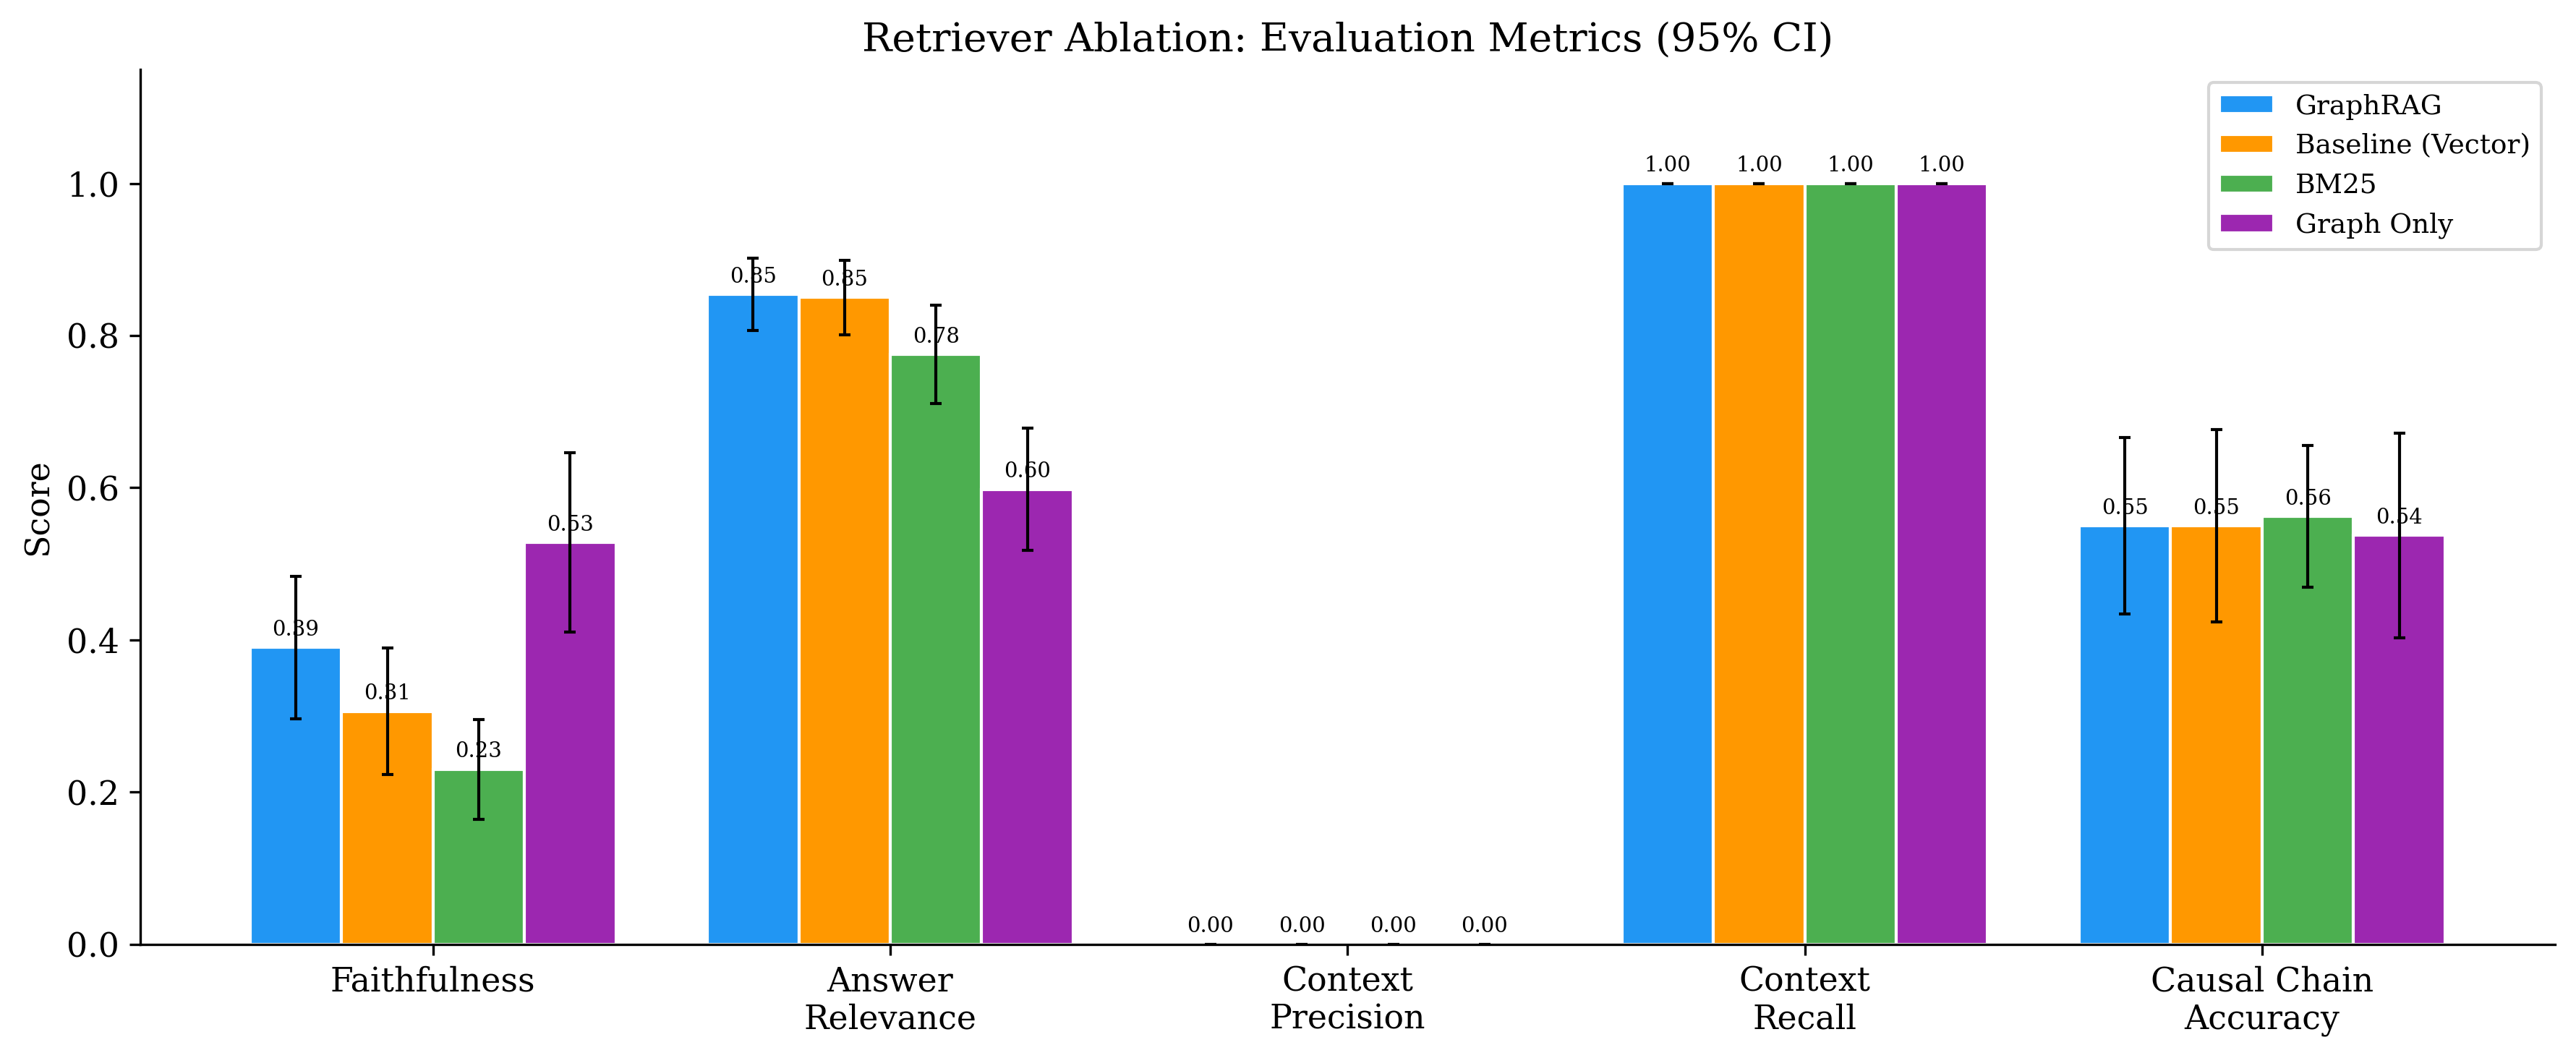
\includegraphics[width=0.92\linewidth]{figures/bar_chart_metrics.png}
\caption{Absolute P@10, nDCG@10, and Ollama faithfulness across the six
retrieval systems.}
\label{fig:bars}
\end{figure}

\begin{figure}[h]
\centering
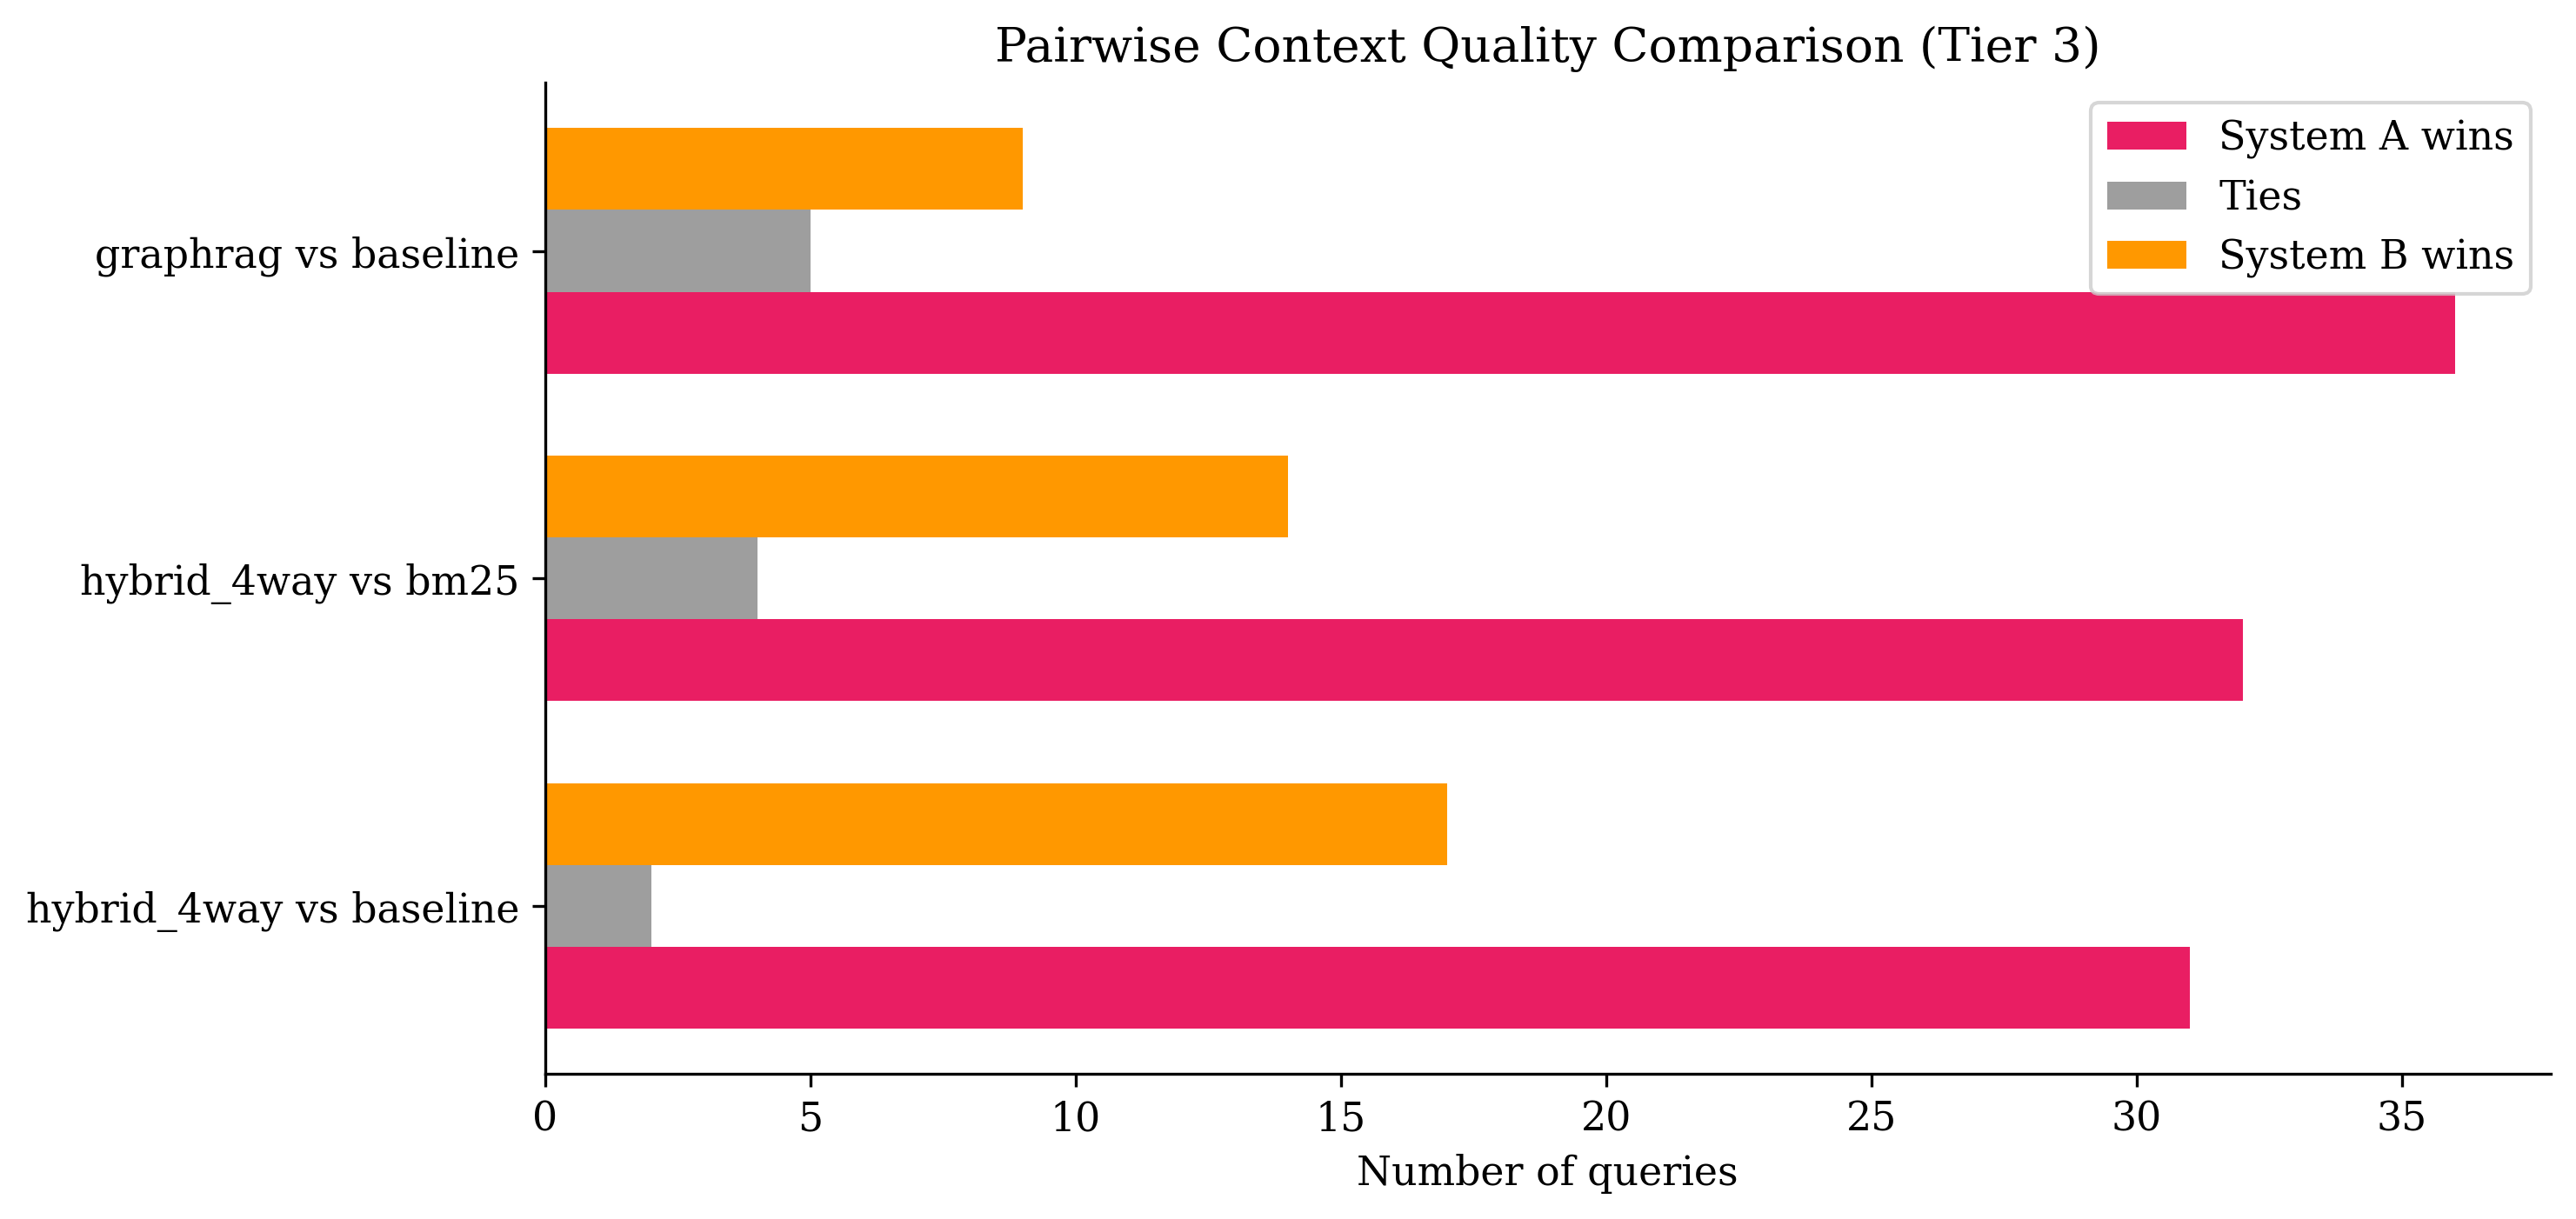
\includegraphics[width=0.78\linewidth]{figures/pairwise_comparison.png}
\caption{Blind pairwise win rates under the Claude judge.}
\label{fig:pairwise}
\end{figure}

\begin{figure}[h]
\centering
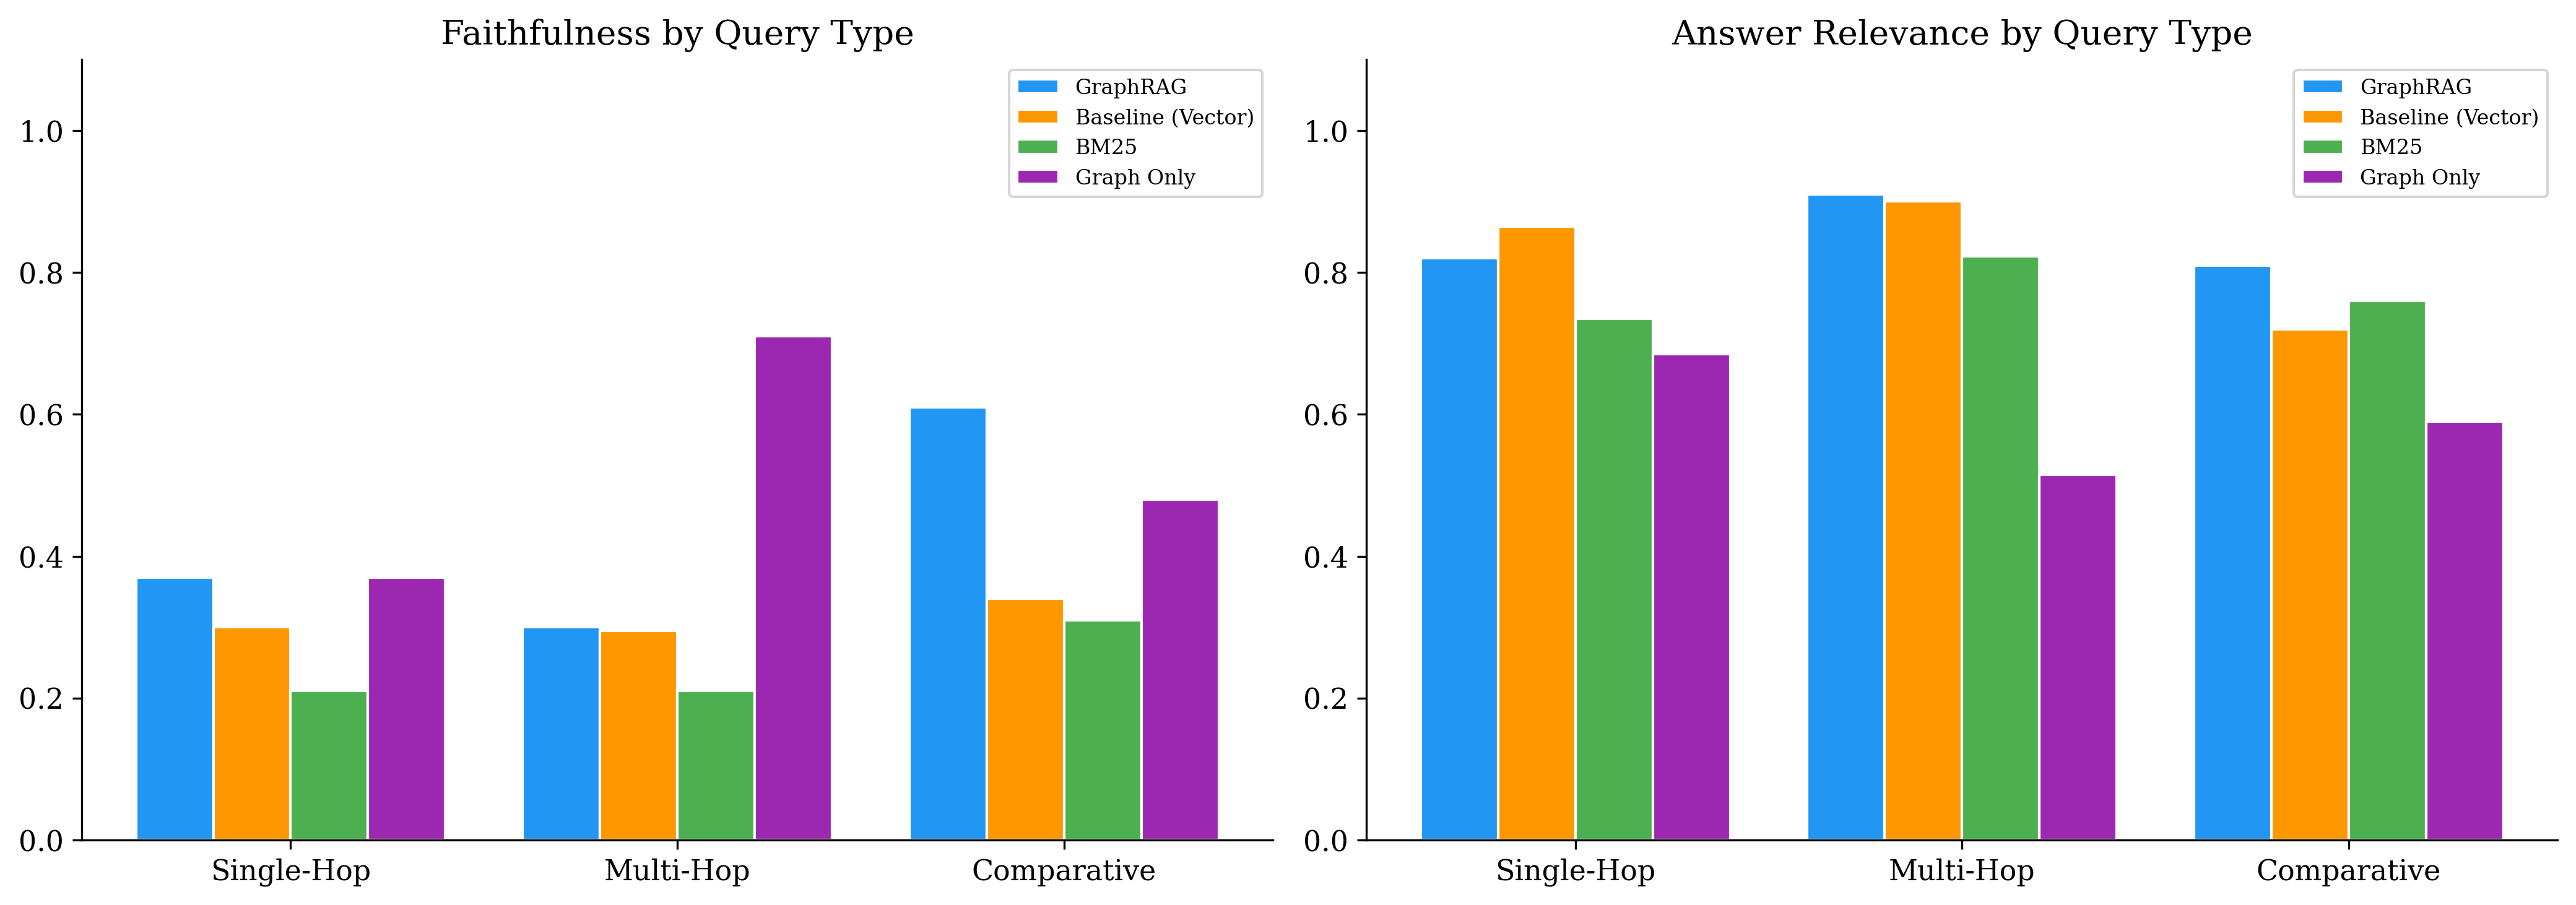
\includegraphics[width=0.88\linewidth]{figures/query_type_breakdown.png}
\caption{Ollama-judged faithfulness by query type.}
\label{fig:querytype}
\end{figure}

\begin{figure}[h]
\centering
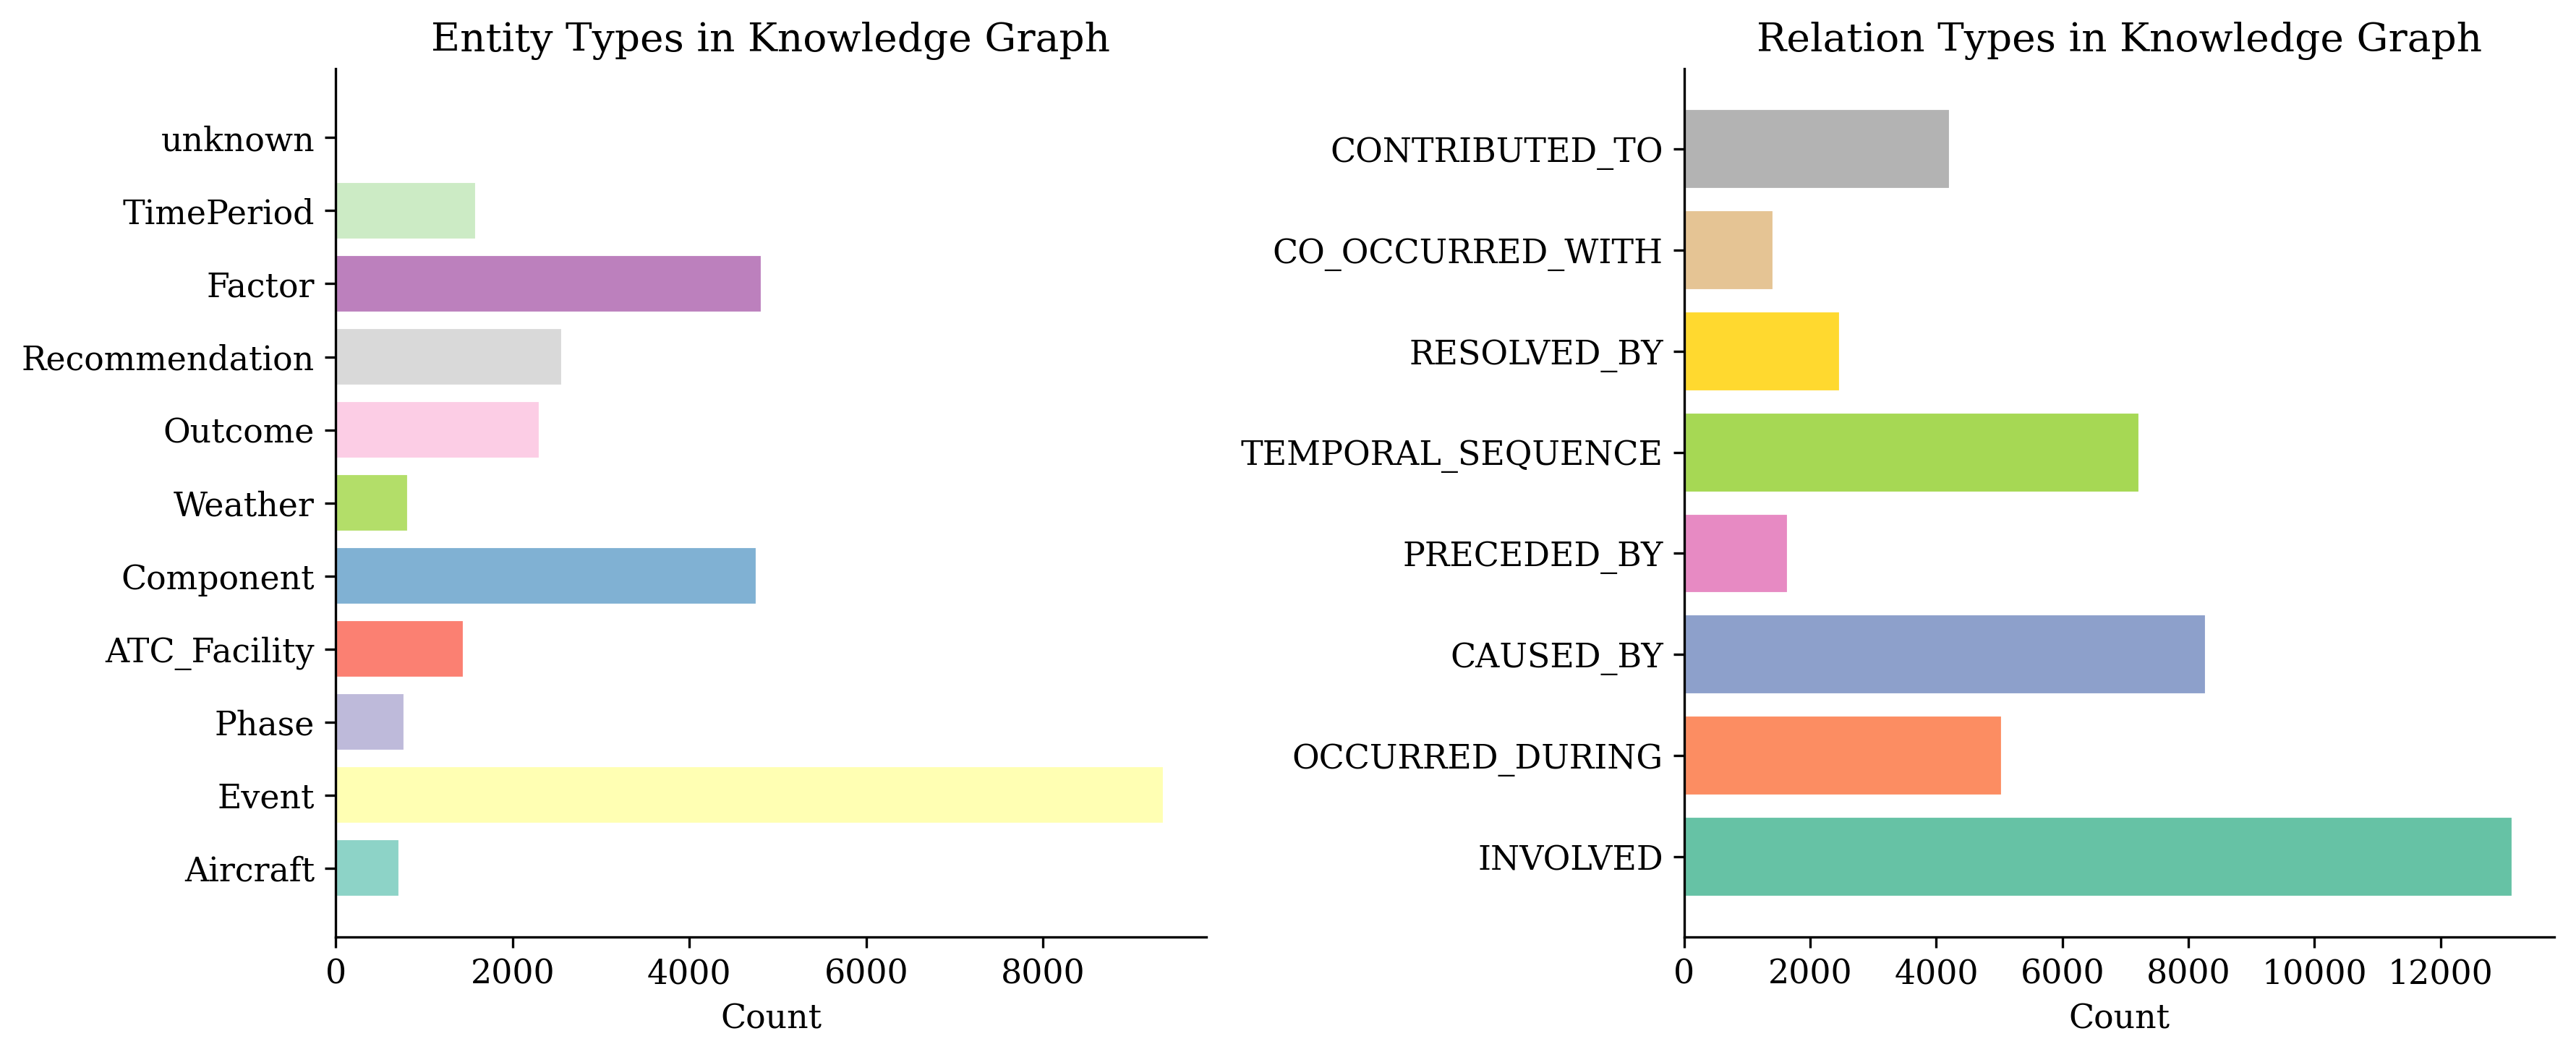
\includegraphics[width=0.78\linewidth]{figures/graph_stats.png}
\caption{Node-type distribution, edge-type distribution, and component-size
histogram pre- and post-canonicalization.}
\label{fig:graphstats}
\end{figure}

% ---------------------------------------------------------------
% 7. Discussion
% ---------------------------------------------------------------
\section{Discussion}
\label{sec:discussion}

\subsection{Retrieval precision is not answer quality}

The most striking finding of our evaluation is not the absolute improvement
of hybrid retrieval over the vector baseline, which is expected given prior
work, but the relationship between PPR-only retrieval and the full $4$-way
hybrid.

PPR alone attains P@10 within $5\%$ of the full hybrid ($0.200$ vs.~$0.210$).
If retrieval precision were the operative quantity for final answer quality,
PPR would be strictly preferred: it is cheaper end-to-end ($2.6$s vs.~$23.1$s),
architecturally simpler (one signal vs.~four), and nearly as precise. Yet
PPR loses on every answer-quality metric under every judge, and decisively
loses pairwise comparisons against the hybrid.

The explanation, we argue, is that PPR's top-$k$ retrieved set is
high-precision at the report level but low-\emph{diversity} at the passage
level. PPR's stationary distribution concentrates on entities connected to
the query, and the reports it selects share those entities. The hybrid's
four signals disagree on which passages rank highest, and this disagreement
functions as diversification. The generator, receiving a more heterogeneous
evidence set, produces answers that are better grounded and more
comprehensively cited.

This phenomenon is known in information retrieval under the label of
\emph{result diversification} \citep{carbonell1998mmr}, but to our knowledge
it has received little attention in the RAG-evaluation literature, where the
implicit assumption is that better retrieval precision monotonically
improves generation quality. Our results suggest otherwise: the correct
target for RAG retrieval is not Top-$k$ precision against a single relevance
oracle, but the coverage-weighted evidence utility of the Top-$k$ set.

\subsection{Reconciling judge disagreement with pairwise preference}

Table~\ref{tab:answer-quality} shows Claude nominally preferring the vector
baseline on faithfulness ($0.410$) over the hybrid ($0.310$).
Table~\ref{tab:pairwise} shows Claude preferring the hybrid $62\%$ of the
time in blind pairwise comparison. These are not contradictions; they are
consistent once one recognizes that the two protocols measure different
quantities.

The pointwise faithfulness protocol asks the judge to score each answer in
isolation on a rubric. Under this protocol, Claude is harsh on answers that
include causal inferences supported by graph edges but not explicitly stated
in any single chunk. Such answers are common in hybrid outputs and rare in
vector-only outputs. The pairwise protocol asks the judge to compare two
answers. Here Claude consistently prefers the more comprehensive hybrid
answer over the narrower vector-only answer. This is not judge failure. It
signals that faithfulness-as-isolated-rubric-score and
faithfulness-as-preference are distinct constructs. Future RAG benchmarks
should report both.

\subsection{Ollama vs. Claude judge gap}

The systematic $0.2$ to $0.4$ faithfulness gap between Ollama and Claude is
substantial. We verified that it is not a prompting artifact: both judges
receive identical rubrics and identical answers. The most likely explanation
is calibration difference. Claude is more conservative about scoring weakly
supported inference as \emph{faithful}, even when the inference is
defensible. System rankings are preserved across judges; the bottom three
systems are ranked identically by both. The gap is primarily an
absolute-scale artifact. We recommend dual-judge reporting as a standard
practice. Absolute single-judge scores risk systematic under- or
over-statement depending on judge choice.

% ---------------------------------------------------------------
% 8. Limitations
% ---------------------------------------------------------------
\section{Limitations}
\label{sec:limitations}

\paragraph{Corpus size.}
The $2{,}000$-report sample may not capture the long-tail distribution of the
full $1.9\text{M}+$ ASRS archive, particularly rare anomaly combinations.

\paragraph{LLM-as-judge variability.}
Absolute faithfulness numbers differ substantially between our two judges.
Single-judge absolute numbers should be interpreted as relative rather than
absolute quality measures.

\paragraph{Evaluation circularity.}
The same model family (Claude Sonnet) is used for entity extraction, answer
generation, and one of the two judges. The second open-weight judge mitigates
but does not eliminate circularity.

\paragraph{Reference answers.}
Reference answers used for relevance computation were generated by Claude
over the full corpus. They are LLM-generated references, not human
gold-standard annotations.

\paragraph{Extraction quality.}
LLM extraction produces graph fragmentation. Three-tier taxonomy
normalization collapses $3{,}766$ components to $186$. Residual fragmentation
of free-text entities, such as human-factor descriptions, remains.

\paragraph{Ontology coverage.}
The $10$-node, $8$-edge ontology is intentionally coarser than ECCAIRS and
CAST. Fine-grained safety analysis would require richer types.

\paragraph{Embedding model.}
\texttt{all-MiniLM-L6-v2} is general-purpose. Domain-specific fine-tuning
would likely improve retrieval for technical aviation terminology.

\paragraph{Temporal reasoning.}
\textsc{TEMPORAL\_SEQUENCE} edges reflect narrative ordering, not
ground-truth timestamps.

% ---------------------------------------------------------------
% 9. Conclusion
% ---------------------------------------------------------------
\section{Conclusion}

We presented \textsc{AeroGraph}, an open implementation of hybrid graph and
vector retrieval over $2{,}000$ real NASA ASRS aviation safety reports,
benchmarked across six retrieval systems with a dual-judge evaluation
protocol. Four-signal Reciprocal Rank Fusion (vector $+$ BM25 $+$ PPR $+$
community summaries) attains the highest retrieval precision
(P@10 $=0.210$, a $84\%$ relative improvement over a vector baseline) and
wins $62$ to $72\%$ of blind pairwise answer-quality comparisons against
single-signal baselines. A more surprising finding is that Personalized
PageRank alone nearly matches the full hybrid on retrieval precision while
losing decisively on answer quality. Signal \emph{diversity}, not the
top-rank precision of any one signal, is the dominant driver of RAG
answer quality. The systematic $0.2$ to $0.4$ faithfulness gap between
local and frontier judges should be reported as a standard part of any
LLM-as-judge evaluation. All code, taxonomy data, benchmark queries, and
per-query judge scores are publicly available.

% ---------------------------------------------------------------
% Bibliography
% ---------------------------------------------------------------
{\small
\bibliographystyle{plainnat}
\bibliography{references}
}

\end{document}
